\chapter{Descripción del problema} \label{ch:descripcion-del-problema}


\section{Definición de conceptos}\label{sec:definicion-de-conceptos}

\subsection{La arquitectura \textit{MIPS}}\label{subsec:la-arquitectura-mips}

Se les conoce con el nombre de \textbf{procesadores \textit{MIPS}} a una familia de microprocesadores que implementan
la arquitectura \textit{RISC} del mismo nombre.
Aunque esta arquitectura no ha tenido un gran éxito en los computadores personales, sí ha gozado de fama en
sistemas embebidos, enrutadores y videoconsolas como la \textit{Nintendo 64} o la \textit{PlayStation 2}. \\

\noindent Su simple diseño y baja curva de aprendizaje hace a esta arquitectura ideal para introducir a los alumnos
a los lenguajes ensamblador.

\subsection{\textit{IDEs}: entornos de desarrollo integrados}\label{subsec:ides-entornos-de-desarrollo-integrados}

Un \textbf{entorno de desarrollo integrado} (\textit{IDE, Integrated Development Environment}) es una aplicación
informática con diversas herramientas usados en el desarrollo, construcción y depuración de \textit{software}.
Un \textit{IDE} suele estar desarrollado con dos objetivos claves en mente: maximizar la productividad del
desarrollador y evitar que este tenga que utilizar herramientas externas en su trabajo.

\noindent Existe una gran variedad de entornos de desarrollos en el mercado.
Estos se pueden clasificar de diferentes maneras.

\noindent \textbf{Según su propósito:}
\begin{itemize}
    \item \textbf{Entornos de desarrollo específicos:} son entornos pensados en el desarrollo en una
    tecnología concreta.
    Algunos ejemplos son \textit{NetBeans}, \textit{CLion} o \textit{Android Studio}.
    \item \textbf{Entornos de desarrollo generales:} son entornos que no se centran en una tecnología en concreto.
    Algunos ejemplos son \textit{Intellij IDEA}\cite{INTELLIJIDEA},
    \textit{Eclipse}\cite{ECLIPSE} o \textit{Microsoft Visual Studio}\cite{VISUALSTUDIO}
\end{itemize}

\noindent \textbf{Según su complejidad:}
\begin{itemize}
    \item \textbf{Entornos de desarrollo complejos:} son aplicaciones pesadas con una gran cantidad de
    características y funcionalidades.
    Algunos ejemplos son \textit{Intellij IDEA},
    \textit{Microsoft Visual Studio} o \textit{Eclipse}.
    \item \textbf{Entornos de desarrollo ligeros:} son aplicaciones que ocupan muy poco espacio, donde
    las características más avanzadas suelen ser componentes descargables.
    Algunos ejemplos son \textit{Visual Studio Code}\cite{VISUALSTUDIOCODE},
    \textit{Atom}\cite{ATOM} o \textit{Notepad++}\cite{NOTEPADPP}.
\end{itemize}

\subsection{Simuladores y emuladores}
\label{subsec:simuladores-y-emuladores}

Tanto los simuladores como los emuladores pueden definirse como un
programa de computador que imita el funcionamiento de uno o varios
componentes \textit{hardware}.
Un emulador o simulador puede imitar una arquitectura, permitiendo
ejecutar aplicaciones ajenas a la arquitectura del computador principal.

\noindent Es importante diferenciar los conceptos de \textbf{simulación}
y \textbf{emulación} a la hora de crear un programa que ejecute
código de arquitecturas externas.
La diferencia entre los simuladores y emuladores se manifiesta
en la manera en la que se implementan.

\noindent Un emulador tiene como objetivo \textbf{imitar el resultado}
que la arquitectura imitada produce al ejecutar un programa, sin tener
en cuenta el proceso interno que produce dicho resultado.
Los emuladores tienden a ser rápidos, intentando producir el resultado
de la manera más rápida y fiel posible.

\noindent Los simuladores tienen como objetivo \textbf{imitar el proceso}
que produce el resultado, simulando todos los componentes de la arquitectura.
Los simuladores tienden a ser más lentos que los emuladores, pero son más
adecuados para desarrollar y depurar aplicaciones para la arquitectura
imitada sin tener el \textit{hardware} físicamente.


\section{Descripción del problema}\label{sec:descripcion-del-problema}

Como se verá más adelante, los simuladores de la arquitectura \textit{MIPS} tuvieron
un auge importante a principios del milenio, con herramientas como \textit{MARS}\cite{MARS}
o \textit{EduMIPS64}\cite{EDUMIPS64}.
Estas herramientas estaban centradas principalmente en el \textbf{ámbito educativo}, proporcionando
interfaces sencillas y pocas herramientas.
Con el paso de los años, estas herramientas han quedado obsoletas, impidiendo desarrollar aplicaciones
en ensamblador \textit{MIPS32} de una manera cómoda.

\noindent Los principales problemas que presentan estas aplicaciones son los siguientes:
\begin{itemize}
    \item \textbf{Falta de herramientas}: los entornos de desarrollo \textit{MIPS} sufren de una
    carencia grave de herramientas importantes.
    Este problema afecta principalmente a programas como \textit{EduMIPS64}, donde no existe un editor de texto y
    el ensamblador es una aplicación separada que require la línea de comandos para funcionar.
    \item \textbf{Falta de estructura de proyecto}: ninguna aplicación actual presenta una estructura
    de proyecto, indispensable para el desarrollo de aplicaciones medianas y grandes.
    \item \textbf{Falta de personalización}: al ser aplicaciones muy sencillas, ninguna permite
    personalizar la apariencia de la interfaz.
    \item \textbf{Obsolescencia}: las aplicaciones están desarrolladas con tecnologías antiguas,
    con interfaces similares a las de los programas de principio de siglo.
    \item \textbf{Falta de capacidad de expansión}: el problema más grave que presentan estas aplicaciones
    es la nula capacidad de expansión de sus características, impidiendo que otros desarrolladores
    añadan nuevas funcionalidades de manera sencilla.
\end{itemize}


\section{Objetivos}\label{sec:objetivos}

El objetivo principal de este proyecto es el desarrollo de \textbf{\textit{JAMS}
(\textit{Just Another MIPS Simulator})}, un \textbf{entorno de desarrollo integrado ligero, expandible y moderno}
centrado en los lenguajes ensamblador y, más concretamente, en el lenguaje ensamblador \textit{MIPS}.

\noindent Específicamente, en este apartado se detallarán diferentes objetivos.

\subsection{Investigar sobre las tecnologías más adecuados para el desarrollo}
\label{subsec:investigar-sobre-las-tecnologias-mas-adecuados-para-el-desarrollo}

La tecnología usada en un proyecto tiene mucho peso en el resultado final.
Es por eso que se debe buscar un conjunto de tecnologías que permitan crear una aplicación
moderna, multiplataforma y expansible.

\noindent Este objetivo puede separarse en dos pasos:
\begin{itemize}
    \item Buscar una lenguaje de programación con capacidad para crear aplicaciones modernas,
    que permita cargar código externo a voluntad y que tenga un buen rendimiento
    tanto en la ejecución como en el desarrollo.
    \item Dentro de las posibilidades del lenguaje de programación seleccionado,
    buscar un \textit{framework} de desarrollo de aplicaciones de escritorio
    que permita desarrollar aplicaciones modernas y de gran calidad.
\end{itemize}

\subsection{Crear un entorno base y un \textit{framework} que permita implementar diferentes herramientas}
\label{subsec:crear-un-entorno-base-y-un-framework-que-permita-implementar-diferentes-herramientas}

\textit{JAMS} pretende ser un entorno de desarrollo completamente modificable.
La mejor manera para conseguir esto es desarrollar una base genérica
que se pueda ajustar posteriormente al desarrollo de una tecnología en concreto.

\noindent Esta base debe poder personalizar cualquier aspecto de la aplicación,
desde poder modificar simples mensajes y parámetros hasta poder
añadir nuevas herramientas.
Estas modificaciones pueden venir de diferentes fuentes, como lo son
los paquetes de idiomas, los paquetes de temas y los complementos.

\noindent Por último, \textit{JAMS} debe permitir al usuario configurar los parámetros
de la aplicación de manera sencilla, proporcionando una interfaz de configuración
cómoda de usar.

\noindent Para conseguir este resultado, se proponen los siguientes subobjetivos:
\begin{itemize}
    \item Desarrollar una aplicación base en conjunto con una \textit{API} que pueda
    ser usada por las diferentes herramientas para tecnologías concretas.
    \item Desarrollar e investigar diferentes formatos que permitan guardar
    y modificar los diferentes elementos estáticos de la aplicación, como lo son
    los idiomas, los temas y la configuración.
\end{itemize}

\noindent Este objetivo está altamente relacionado con los
objetivos principales del Trabajo de Fin de Grado del Grado en
Diseño y Desarrollo de Videojuegos: desarrollar un \textbf{sistema de carga
dinámica de componentes}, permitiendo al usuario activar y desactivar
componentes a voluntad sin tener que reiniciar la aplicación y
desarrollar tecnologías que permitan \textbf{modificar}
todos los aspectos de \textit{JAMS} mediante componentes.
Aunque los objetivos de los dos Trabajos de Fin de Grado están
correctamente definidos, los procesos de desarrollo para lograrlos están
fuertemente vinculados.
Es por este motivo por el que se mencionará mucho la idea de \textbf{componente}
(un programa externo que modifica el comportamiento de una aplicación principal),
aunque ninguno de los objetivos de este Trabajo de Fin de Grado requiera el
desarrollo de estos.

\subsection{Desarrollar un entorno de desarrollo para la arquitectura \textit{MIPS32}}
\label{subsec:desarrollar-un-entorno-de-desarrollo-para-la-arquitectura-mips32}

Una vez se tenga una base sólida, se ha de desarrollar un editor, un ensamblador
y un simulador para la arquitectura \textit{MIPS32r6}.
Estas tres tecnologías se apoyarán en diferentes herramientas que complementarán
su utilización, como puede ser el caso del explorador en el editor y el visualizador
de memoria en el simulador.

\noindent Este objetivo se desarrollará en dos pasos:

\begin{itemize}
    \item Desarrollar un editor, un ensamblador y un simulador usando la tecnología
    proporcionada por la base.
    Estos tres componentes deben ser expandibles mediante componentes externos.
    \item Desarrollar diferentes herramientas que complementen las funcionalidades
    del editor, del ensamblador y del simulador.
\end{itemize}

\noindent Cabe destacar que no es un objetivo el permitir crear código válido para
entornos \textit{MIPS} reales.

\section{Metodología}\label{sec:metodologia}

Debido a que la aplicación está dividida en tres secciones (tecnologías, base y entorno de desarrollo \textit{MIPS}),
es muy importante marcar una metodología que permita un desarrollo consistente, eficiente y rápido.
A nivel de desarrollo se ha optado por una metodología ágil, con \textit{sprints} de varios meses
donde se desarrollan una serie de características claves.
Todas las características se someten a varias iteraciones donde se modifican y mejoran hasta lograr un
buen resultado.

\noindent También se ha seguido un desarrollo basado en pruebas unitarias,
permitiendo mantener la calidad del código mientras la aplicación va evolucionando.

\noindent Toda la metodología ha sido implementada mediante las herramientas proporcionadas por \textit{GitHub}.
Los estados de las características asignadas a un \textit{sprint} son documentados mediante proyectos.
Las acciones obligan a que las pruebas unitarias deban superarse sin errores si se desea añadir una nueva
característica a la rama principal.
Estas acciones también se emplean para generar los binarios cuando un \textit{sprint} es superado y una
nueva versión de \textit{JAMS} es lanzada.

\begin{figure}[H]
    \centering
    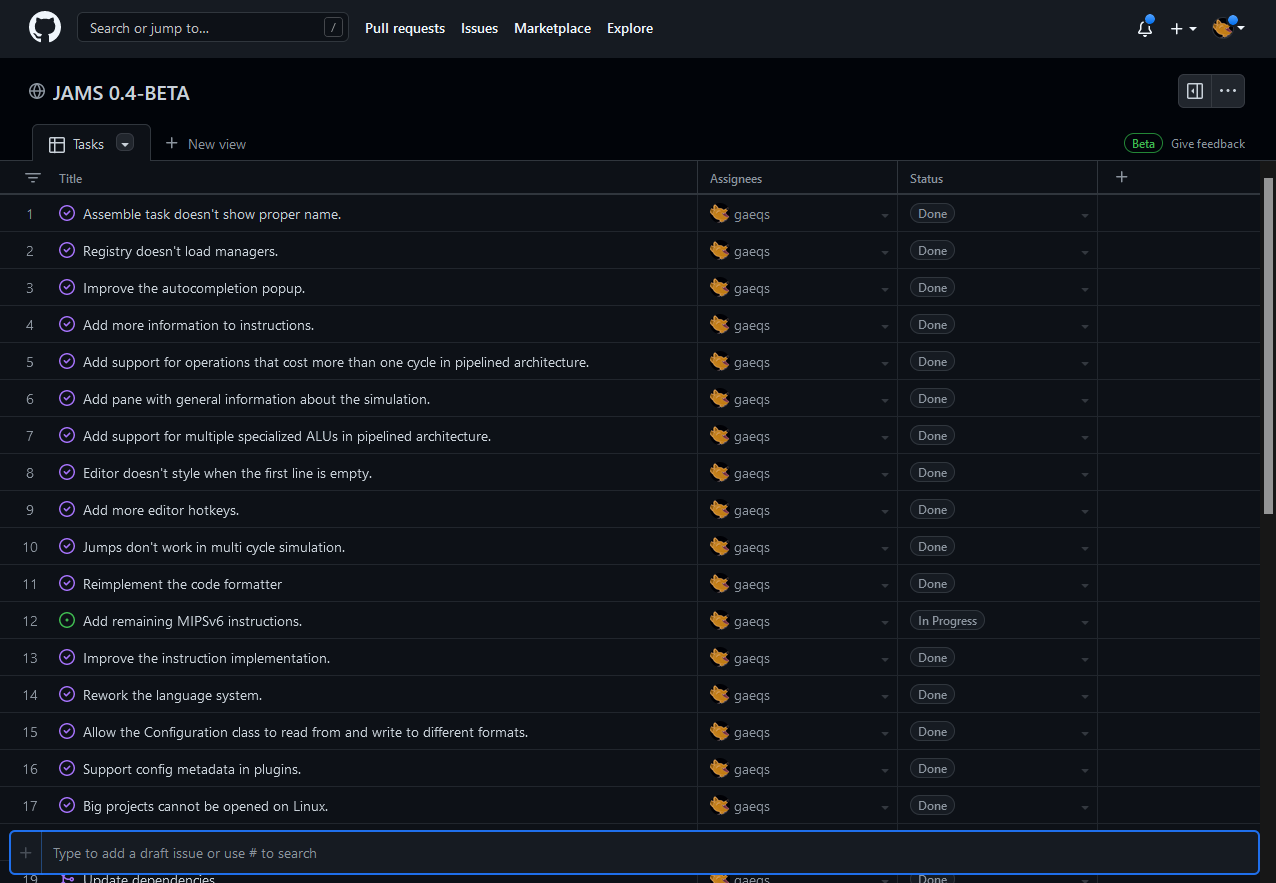
\includegraphics[width=\textwidth]{images/introduction/github}
    \caption{Proyecto de \textit{GitHub} para la versión 0.4-BETA}
    \label{fig:introduccion-github}
\end{figure}